\chapter{Isotropic simulation of the High Energy Telescope with the Solar Orbiter spacecraft model}
\label{chp:HETSimulation}

To simulate the response of the High Energy Telescope (HET, \autoref{sec:solohet}), part of the Energetic Particle Detector \citep[EPD][]{RodriguezPacheco-2019-EPD} onboard Solar Orbiter (SolO), for an isotropic radiation field, a simulation using the GEometry And Tracking 4 \citep[Geant4][]{Agostinelli-2003} was performed. GEANT4 is a software toolkit developed at CERN for Monte Carlo simulations of the interaction of particles with matter, and is widely used in many different fields. A Geant4 simulation typically requires the definition of a particle source (e.g. a particle beam, a surface or volume source), a model of the geometry and materials of the experimental setup, and one or more sensitive detectors in which particle hits are detected. A so-called ``physics list'' describes all possible interaction processes and their probabilities, from which Geant4 then chooses stochastically for each simulated particle. As a result, the trajectory of each particle and the detected particles in each detector can be stored and used processed to calculate e.g. the response function of a particle detector.

This simulation builds on top of the work by \citet{Elftmann-2020-PhD}, who simulated the nominal data products of HET with Geant4. In this case, particles were simulated only from a circular source in front of the A detector \citet[Figure 5.1]{Elftmann-2020-PhD}, which fills the nominal field of view (FOV) of HET. However, particles entering HET from outside its FOV may also play a role for certain data products, especially for single-detector counters, which are sensitive to particles entering the telescope from all directions (e.g., through the housing). These counters were used by \citet{Forstner-2021-SolO} to observe Forbush decreases with HET. Thus, it makes sense to simulate the HET detector in an isotropic particle flux to model its response to Galactic Cosmic Rays (GCRs), and this will be done in \autoref{sec:isotropic_sim}.

For an isotropic particle flux, it is also important to take into account the Solar Orbiter spacecraft that HET is mounted on. This is less relevant for the nominal FOV, as the HET telescopes are oriented so that their openings do not point towards the spacecraft body (i.e. tangential to an edge of the body). But for single detector counters, particles coming from the solid angle covered by the spacecraft can be shielded away, or may generate secondaries that are then detected within HET. This will be investigated in \autoref{sec:spacecraft_model}.

\section{Isotropic simulation of HET}
\label{sec:isotropic_sim}

For the isotropic simulation, the geometric model of the HET instrument and its electronics box were reused from the simulation by \citet{Elftmann-2020-PhD}, so the reader is referred to this work for further details about its definition. The simulation setup was also very similar to \citet{Elftmann-2020-PhD}, using Geant4 version 10.1.2 with the pre-defined general-purpose physics list \texttt{QGSP\_BERT}, and a power law spectrum for the energy-dependent intensity $I$ of the input particles:
\begin{equation}
I(E) \sim E^{-1}
\end{equation}
This makes it possible to simulate the same number of particles in each primary energy bin when the bins are logarithmically spaced. Only protons between \SI{5}{\mega\electronvolt} and \SI{100}{\giga\electronvolt} were simulated as input particles in this case, as other species were neglected in the modeling approach of \citet{Forstner-2021-SolO}. Still, all secondary particles generated by these primary protons are taken into account in the output of simulation. Of course, other primary species such as electrons and heavy ions can be simulated in a similar fashion in the future.

In contrast to the circular planar source surface used by \citet{Elftmann-2020-PhD}, a spherical source with a radius of \SI{15}{\centi\meter} (large enough to surround HET and its electronics box) was defined, and particles were injected following a cosine-law angular distribution. This represents an isotropic flux entering HET from all sides.
The simulation was run for \num{5e8} particles, and $\sim\num{1.6e7}$ particle hits (primary or secondary) were registered in the HET detectors.

\section{The spacecraft model}
\label{sec:spacecraft_model}

To simulate how the interaction of GCR particles with the Solar Orbiter spacecraft affects the HET measurements, the spacecraft needs to be included into the Geant4 simulation. Accurately modeling a spacecraft is notoriously difficult, as it consists of numerous components and information about their exact shape and composition is not always readily available. Thus, simulations taking into account spacecraft effects often need to make many assumptions and drastically simplify the geometry of the spacecraft (see e.g. \citet{Appel-2018-PhD,Appel-2018} for a similar simulation of the Mars Science Laboratory rover).

In the case of Solar Orbiter, ESA has provided a computer-aided design (CAD) model of the spacecraft that can serve as a reference for simulations (D. Müller, 2020, priv. comm.). This file (\texttt{dpl7a1\_bulk.bdf}) is provided in the NASTRAN BDF format
and contains the 3D geometry of the spacecraft, including material properties such as the density. Using the freeware software \textit{FEX}\footnote{\url{http://www.f-e-x.com/}}, it is possible to inspect the model and measure the dimensions and total mass of certain structures.

As shown in \autoref{fig:solo_spacecraft_model}, the model accurately represents the major structures of the SolO spacecraft, such as the main body, the solar panels, the heat shield, the instrument boom and various communications and radio wave antennae. However, not all parts are modeled in detail: Many small structures, such as the scientific payload and electronics within the spacecraft body, are replaced with mass points that are attached to the model (shown as colored tetrahedra in the image), and thus no information about their extent and materials are provided. In addition, some parts of the spacecraft are constructed using composite materials, such as honeycomb structures instead of solid Aluminium --- in these cases, the material properties given in the CAD file do not include the correct density, but are instead set to zero. Thus, the total mass of the spacecraft according to the CAD file is \SI{1202}{\kilogram}, which is significantly less than the total launch mass off $\sim\SI{1800}{\kilo\gram}$, or $\sim\SI{1600}{\kilo\gram}$ without fuel \citep{Mueller-2020-SolO}.

\begin{figure}
	\centering
	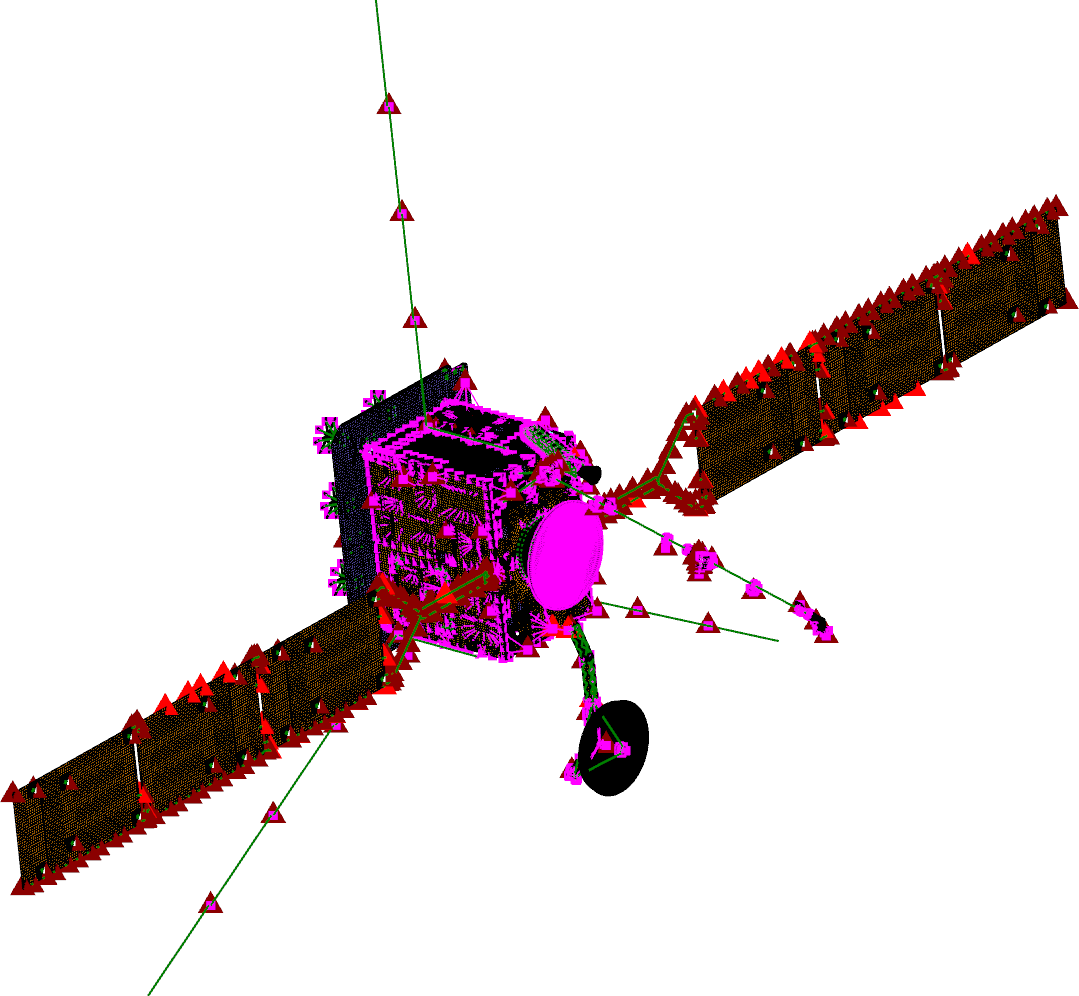
\includegraphics[width=0.7\linewidth]{images/solo_spacecraft_model}
	\caption[Density model of the Solar Orbiter spacecraft]{Density model of the Solar Orbiter spacecraft as supplied by ESA. Colored tetrahedra correspond to mass points that are inserted into the model as a replacement for structures whose geometry is not modeled (e.g. scientific payload).}
	\label{fig:solo_spacecraft_model}
\end{figure}

An automated conversion from the CAD file to a Geant4-compatible model (GDML) is not easily possible and would also not be very meaningful due to the shortcomings of the CAD model described above.
As a first step towards implementing the spacecraft model in Geant4, I have therefore simply measured the dimensions of the main box-shaped spacecraft body in the CAD file and created a corresponding box in Geant4. To estimate the mass of this box, the following estimations are made: 
The total mass of the two solar panels in the CAD file is \SI{110}{\kilo\gram}, so the main spacecraft body (without solar panels) has a mass of $\sim\SI{1100}{\kilogram} + \SI{600}{\kilogram} = \SI{1700}{\kilogram}$ (adding the \SI{400}{\kilogram} of mass that is ``missing'' in the CAD file \SI{200}{\kilogram} of fuel). This value is used as the mass of the box in the Geant4 model.
For the material of the box, we assume that the mass is equally distributed throughout the box, with \SI{200}{\kilogram} of hydrazine fuel, and the remaining mass split 50:50 between electronics components and aluminium (\SI{750}{\kilogram} each). Electronics were modeled using the PCB material taken from \citet{Appel-2018,Appel-2018-PhD}.
The dimensions and materials used are summarized in \autoref{tab:solo_spacecraft_gdml}.

\begin{table}
    \begin{tabular}{rp{6cm}}
        \toprule
        \multicolumn{2}{c}{\textbf{SolO spacecraft body}}                   \\
        \midrule
        X dimension & \SI{1812}{\milli\meter}                \\
        Y dimension & \SI{1461}{\milli\meter}                \\
        Z dimension & \SI{2200}{\milli\meter}                \\
        Mass        & \SI{1700}{\kilogram}                   \\
        Density     & \SI{291.89}{\kilogram\per\cubic\meter} \\
        Composition & \SI{12}{\percent} Hydrazine (N$_2$H$_4$) \newline \SI{44}{\percent} PCB material (see right table) \newline \SI{44}{\percent} Aluminium Alloy (same as HET housing) \\
        \bottomrule
    \end{tabular}
    \hspace{1cm}
    \begin{tabular}{rr}
    	\toprule
    	\multicolumn{2}{c}{\textbf{PCB material}} \\ \midrule
    	Cu      & \SI{20}{\percent}     \\
    	SiO$_2$ & \SI{15}{\percent}     \\
    	PET     & \SI{9.9}{\percent}    \\
    	PP      & \SI{4.8}{\percent}    \\
    	Al      & \SI{2}{\percent}      \\
    	Pb      & \SI{2}{\percent}      \\
    	Ni      & \SI{2}{\percent}      \\
    	Fe      & \SI{8}{\percent}      \\
    	Sn      & \SI{4}{\percent}      \\
    	Mg      & \SI{30}{\percent}     \\ \bottomrule
    \end{tabular}
    \caption{Details of the spacecraft model used for the HET simulation. The left table shows the dimensions and composition of the box-shaped spacecraft body, while the right table shows the PCB material taken from \citet{Appel-2018,Appel-2018-PhD}.}
    \label{tab:solo_spacecraft_gdml}
\end{table}

HET was then positioned next to the spacecraft body, at a location derived from the position of the corresponding mass point of HET 1 in the CAD file, and with the correct orientation relative to the Sun. As both HET 1 and HET 2 are located at an edge of the spacecraft body, the difference between the positions of HET 1 and HET 2 is not expected to be significant for an isotropic radiation field --- but of course, this may be verified with another simulation in the future. As a source, a cube of edge length \SI{260}{\centi\meter}, which surrounds the spacecraft body and the HET sensor was used, again with a cosine-law distribution of particles injected from its surface.

To speed up future simulations, the spacecraft model may also be converted into spherical shells of equivalent column density that are placed around the HET sensor. In this case, the source size could be significantly reduced and thus the fraction of simulated particles that reach HET would increase. The simulation results with the actual spacecraft geometry can then be used to validate this approach.

\section{Analysis of the simulation results}

For the study by \citet{Forstner-2021-SolO}, the 